%  --------------------------------------------------------------------------
%  Diplomarbeit Dokumentation
%  Created by Silvan Spross on 2011-04-02.
%  --------------------------------------------------------------------------

%  --------------------------------------------------------------------------
%  Latex Document Settings
%  --------------------------------------------------------------------------
\documentclass[
11pt, % Schriftgrösse
a4paper, % A4 Papier
BCOR10mm, % Absoluter Wert der Bindekorrektur, z.B. BCOR1cm
DIV14, % Satzspiegel festlegen siehe
       % http://www.ctex.org/documents/packages/nonstd/koma-script.pdf
footsepline = false, % Trennlinie zwischen Textkörper und Fußzeile
                     % bei normalen Seiten
headsepline, % Trennlinie zwischen Kopfzeile und Textkörper
             % bei normalen Seiten
oneside, % Zweiseitig
openright,
halfparskip, % Europäischer Satz mit Abstand zwischen den Absätzen
abstracton, % inkl. Abstract
listof=totocnumbered, % Abb.- und Tab.verzeichnis im Inhaltsverzeichnis
bibliography=totocnumbered % Lit.zeichnis in Inhaltsverzeichnis aufnehmen
]{scrreprt}

\usepackage[automark]{scrpage2} % Gestaltung von kopf- und Fußzeile
\usepackage[ngerman]{babel}
\usepackage[ngerman]{translator}
\usepackage{tocbasic}
\usepackage[utf8]{inputenc}
\usepackage{lmodern} % Latin Modern
\usepackage[T1]{fontenc}
\usepackage{hyphenat}
\usepackage{ae} % Schöne Schriften für PDF-Dateien

% Tradmark
\def\TTra{\textsuperscript{\texttrademark}}

%1.5 Zeilenabstand
\usepackage[onehalfspacing]{setspace}

% Festlegung des Seitenstils (scrpage2)
\pagestyle{scrheadings}
\clearscrheadfoot
\automark[chapter]{section}

% \lehead{\sffamily\upshape\headmark}
% \cehead{}
% \rehead{}
% \lefoot[\pagemark]{\upshape \pagemark}
% \cefoot{}
% \refoot{}
% \lohead{}
% \cohead{}
\lohead{\sffamily\upshape\headmark}
\lofoot{}
\cofoot{}
\rofoot[\pagemark]{\scshape \pagemark}

% Surround parts of graphics with box
\usepackage{boxedminipage}

% Package for including code in the document
\usepackage{listings}

% If you want to generate a toc for each chapter (use with book)
\usepackage{minitoc}
\usepackage{longtable}

% Abkürzungsverzeichnis erstellen.
\usepackage[printonlyused]{acronym}

% schöne Tabelle zeichnen
\usepackage{booktabs}
\renewcommand{\arraystretch}{1.4} %Die Zeilenabstände in Tabllen angepasst.

% für variable Breiten
\usepackage{tabularx}

% Durchgestrichener Text
\usepackage[normalem]{ulem} %emphasize weiterhin kursiv

% This is now the recommended way for checking for PDFLaTeX:
\usepackage{ifpdf}

\usepackage[hyperfootnotes=false]{hyperref}
\hypersetup{
  bookmarks=true,         % show bookmarks bar?
  unicode=true,           % non-Latin characters in Acrobat’s bookmarks
  pdftoolbar=true,        % show Acrobat’s toolbar?
  pdfmenubar=true,        % show Acrobat’s menu?
  pdffitwindow=true,      % window fit to page when opened
  pdfstartview={FitH},    % fits the width of the page to the window
  pdftitle={Diplomarbeit},   
  pdfauthor={Silvan Spross},
  pdfsubject={Definition und Optimierung der Projektprozesse bei allink.creative},
  pdfcreator={TeX Live 2009},
  pdfproducer={pdfTeX, Version 3.1415926-1.40.10},
  pdfnewwindow=true,      % links in new window
  colorlinks=true,       % false: boxed links; true: colored links
  linkcolor=blue,          % color of internal links
  citecolor=green,        % color of links to bibliography
  filecolor=magenta,      % color of file links
  urlcolor=cyan          % color of external links
  % linkcolor=black,          % color of internal links
  % citecolor=black,        % color of links to bibliography
  % filecolor=black,      % color of file links
  % urlcolor=black          % color of external links
}

\ifpdf
    \usepackage[pdftex]{graphicx}
\else
    \usepackage{graphicx}
\fi

\makeatletter 
\let\orgdescriptionlabel\descriptionlabel 
\renewcommand*{\descriptionlabel}[1]{% 
  \let\orglabel\label 
  \let\label\@gobble 
  \phantomsection 
  \edef\@currentlabel{#1}% 
  %\edef\@currentlabelname{#1}% 
  \let\label\orglabel 
  \orgdescriptionlabel{#1}% 
} 
\makeatother 

%  --------------------------------------------------------------------------
%  Start Document
%  --------------------------------------------------------------------------
\title{Definition und Optimierung der Projektprozesse bei allink.creative}

\author{Diplomarbeit in Informatik\\
    \\
    Studierender - Silvan Spross\\
	Auftraggeber - Michael Walder\\
    Projektbetreuer - Beat Seeliger\\
    Experte - tbd\\
	\\
	HSZ-T - Technische Hochschule Zürich}

\date{März 2011 bis Juni 2011}

\begin{document}

  \ifpdf
    \DeclareGraphicsExtensions{.pdf, .jpg, .tif}
  \else
    \DeclareGraphicsExtensions{.eps, .jpg}
  \fi
  
  \pagenumbering{Alph}
  
  \maketitle
  \cleardoublepage

  \begin{abstract}
tbd
\end{abstract}
  \cleardoublepage

  \pagenumbering{roman}
  
  \tableofcontents
  \cleardoublepage
  
  \pagenumbering{arabic}
  
  \chapter{Einführung}
  \section{Motivation}
Das Schreiben einer Diplomarbeit bedeutet nebst dem baldigen Abschluss des Studiums
auch einen enormen Aufwand. Deshalb ist die Wahl des Themas und meine
Motivation in diese Arbeit die nötige Zeit und Qualität zu investieren enorm
wichtig. Aus diesem Grund möchte ich kurz erläutern, was mich zu dieser
Arbeit geführt hat.

Ein eigenes Unternehmen zu gründen und erfolgreich zu führen war schon immer
einer meiner Träume. Nach meiner Lehre im Jahre 2004 machte ich mich deshalb
selbstständig und gründete 2005 die SiSprocom GmbH\footnote{\url{http://sisprocom.ch/}}. 
Im ersten Jahr bestanden
die Tätigkeitsfelder überwiegend aus Webdesign und Schulungen. Im Bereich
Webdesign lag der Fokus hauptsächlich auf der Programmierung. Dieser Bereich 
entwickelte sich immer stärker in Richtung 
Applikationsentwicklung und dank Aufträge einer Zürcher Grossbank 
lag der Fokus bald nur noch darauf.

Durch dieses grössere Mandat wuchs die SiSprocom GmbH zwischenzeitlich
auf 3 Mitarbeiter. Dies führte zu massiv mehr Aufwand in der Administration
und schnell wurde klar, dass zwingend Stunden rapportiert und das Schreiben
von Rechnungen vereinfacht werden musste. Wir bedienten uns damals Google 
Docs\footnote{\url{http://docs.google.com/}} um die rapportierten Stunden zentral zu 
verwalten und einer selbst geschriebenen Software um vereinfacht Rechnungen 
verwalten und schreiben zu können.
So lehrreich und spannend die Arbeit in dieser Grossbank auch war, so kompliziert
waren auch ihre Abläufe und Prozesse. Zu diesem Zeitpunkt schwor ich mir, dies
in meiner Unternehmung einmal besser zu lösen.

Ende 2009 realisierte ich, dass ich zwar ein eigenes Unternehmen hatte und
selbständig war, jedoch fast ausschliesslich für einen Kunden arbeitete.
Ich kam zum Schluss, dass dies nicht mein eigentliches Ziel meiner Selbständigkeit 
war und begriff
relativ schnell, dass ich mich von dieser Abhängigkeit nur lösen konnte, wenn
ich mich vollständig aus diesem Mandat zurückziehe.
Dies tat ich dann anfangs 2010 auch und mietete ein Büro in den Räumlichkeiten
der allink GmbH\footnote{\url{http://allink.ch/}}. Deren IT hatte zu diesem Zeitpunkt 
ein paar grössere
Herausforderungen zu bewältigen und ich bot meine Hilfe an. Schnell wurde
daraus eine Partnerschaft und die SiSprocom fusionierte mit der allink.
Heute im März 2011, knapp ein Jahr danach, ist Die SiSprocom GmbH um 30\% 
gewachsen und arbeitet ausschliesslich für die erwähnte Grossbank. Alle anderen Projekte
haben wir in die allink GmbH übernommen. Die administrativen Aufgaben der
SiSprocom GmbH wurden
meinem Vater abgegeben, der zusammen mit einem Treuhänder das laufenden
Mandat und die drei Mitarbeiter gut handhaben kann. So konnte ich mich ganz
auf die neuen Herausforderungen bei der allink konzentrieren.
Die allink GmbH ist inzwischen um 70\% auf 17 Mitarbeiter gewachsen und muss sich dadurch
neuen Herausforderungen in der Organisation und Projektabläufe stellen.

Da mich die Selbständigkeit auch durch das ganze Studium begleitet hat, möchte 
ich meine Diplomarbeit nutzen um unser Unternehmen zu optimieren.

\section{Zielsetzung}
Mir und den anderen drei Partnern bei der allink GmbH ist klar, dass unser
heutiger Projektablauf nicht optimal ist. Zu oft sehen wir uns mit gleichen
Problemen konfrontiert, die in anderen Projekt schon einmal gelöst wurden.
Jedes Mal versucht man daraus zu lernen, ohne etwas konkret festzuhalten oder
wirklich zu verändern. Das liegt meist daran, dass zu viel ansteht und man
die internen Verbesserungen hinter die Aufträgen und Wünschen der Kunden
stellt.
Mein Ziel ist es mit Hilfe dieser Arbeit den aktuellen Projektablauf der
allink GmbH genauer zu untersuchen und auf dessen Vorteile und Nachteile einzugehen.
Danach versuche ich die eigentlichen Anforderungen der verschiedenen Stakeholder
unseres Projektablaufes aufzunehmen und Kennzahlen zu definieren, die in Zukunft
bei einem verbesserten Projektablauf erfüllt und gemessen werden sollen.
Daraus erarbeite ich Varianten des neuen Projektablaufes und versuche auch
diese so zu bewerten, dass die allink GmbH als mein Auftraggeber einen
Entscheid fällen kann, welchen Projektablauf man in Zukunft einsetzen und 
verfeinern möchte. Der neue Projektablauf soll abschliessend in einem ``Proof of Concept'', also
anhand eines konkreten Projektes, getestet werden. Natürlich wird ein einziger
``Proof of Concept'' nicht ausreichen um vollständig sicherzustellen, dass der
neue Projektablauf optimal ist. Dies wird sich aber dann im Laufe der Zeit zeigen.

Für mich ist das Ziel meiner Diplomarbeit erreicht, wenn ich unserer Firma anhand der Analyse und
dem Aufzeigen von Problemen und möglichen Lösungen helfen könnte, den täglichen
Ablauf unserer Projekte für alle Parteien angenehmer und effizienter zu gestalten.
Das beinhaltet natürlich auch alle erwarteten Resultate\footnote{Die erwarteten 
Resultate sind in der Aufgabenstellung im Anhang \ref{chap:aufgabenstellung} ersichtlich.}, die ich mir in meiner
Aufgabenstellung der Diplomarbeit gestellt habe.
  
  \cleardoublepage
  
  \chapter{Analyse}
  \section{Vorgehensmodell nach Grochla}
Zur Erstellung meiner Ist-Analyse verwende ich die ersten drei Phasen des 
Vorgehensmodell von Erwin Grochla\cite[S. 44-74]{grochla1982grundlagen}.
Die weiteren vier Phasen führen über eine Analyse hinaus und kommen
nicht zur Anwendung.

\subsection{Voruntersuchung}
In der Voruntersuchung, auch Pilotstudie genannt, stellt man sich Fragen wie
``Was soll geändert werden?'' und ``Welches sind die Ziele?''. Man verschafft
sich einen Grobüberblick über das eigentliche Problem und die Rahmenbedingungen
möglicher Lösungen. Auch entscheidet man in der Voruntersuchung, ob der Prozess
fortgesetzt oder abgebrochen werden soll. In der Voruntersuchung können die 
meisten Analyse- und Bewertungstechniken verwendet werden.

Nach Absprache mit dem Auftraggeber werde ich mir zur Voruntersuchung mit  
Hilfe von MindMaps einen besseren Überblick über die aktuellen Probleme bei
allink verschaffen. Auf die einzelnen Punkte soll genauer eingegangen
und wenn möglich Fallbeispiele aus der Praxis genannt werden.

Ich verwende die Technik der MindMaps schon seit einigen Jahren und verwende
sie sehr oft in Projekten um mir einen Überblick über Themen zu verschaffen.

\begin{quotation}
Eine Mind-Map beschreibt eine besonders von Tony Buzan geprägte kognitive 
Technik, die z.B. zur Erschliessung und visuellen Darstellung eines Themengebietes, 
zur Planung oder für Mitschriften genutzt werden kann. Hierbei soll das Prinzip 
der Assoziation helfen, Gedanken frei zu entfalten und die Fähigkeiten des Gehirns 
zu nutzen. Die Mind-Map wird nach bestimmten Regeln erstellt und gelesen. Den 
Prozess bzw. das Themengebiet bzw. die Technik bezeichnet man als Mind-Mapping.
\cite{wikipedia_mindmap}
\end{quotation}

\subsection{Ist-Aufnahme}
In der zweiten Phase erfasst man den aktuellen Zustand indem man das zu 
Untersuchende aus möglichst vielen Betrachtungswinkeln analysieren. Zu den
Techniken der Ist-Aufnahme zählen die Selbstaufschreibung, die Befragung und 
die Beobachtung.

Ich werde mit mir selbst eine Selbstaufschreibung durchführen, da ich in meinem 
Arbeitsalltag unseren Problemen genau so ausgesetzt bin. Aber da mir nur begrenzt
Zeit zur Verfügung steht und damit die Mitarbeiter möglichst ungestört arbeiten
können, begrenze ich Befragungen auf die Partner. Die Meinungen und Beobachtungen
aller Partner fliesst dann in die Ist-Aufnahme ein.

\subsection{Ist-Kritik}
In der dritten Phase widmet man sich den erhobenen Informationen aus der zweiten Phase. 
Die genauen Ursachen der Probleme sollen herausgeschält werden, damit nicht nur 
Symptome behandelt werden. 

Um die Probleme auf ihre tatsächlichen Ursachen zurückführen zu können,
werde ich eine Form der Prüfmatrix, eine Problem-Ursachen Matrix, erstellen.

\begin{quotation}
    Die Prüfmatrix ist ein vereinfachtes Verfahren um Mängel und deren Ursachen 
    zu ermitteln. Mängel werden dabei möglichen Ursachenkategorien matrixförmig 
    gegenübergestellt. Im Schnittpunkt von Mangel und Ursachenkategorie werden 
    die tatsächlichen Ursachen gesucht.\cite{schmidt2000methode}
\end{quotation}

\section{Voruntersuchung}
\subsection{Überblick}
Man hat sich bei allink bis heute noch nicht richtig mit dem eigenen Organigramm
auseinander gesetzt. Zur Zeit existiert nur die Unterscheidung zwischen Mitarbeitern 
und Partnern, aus denen sich gleichzeitig die Geschäftsleitung zusammen setzt.

\begin{figure}[htbp]
\begin{center}
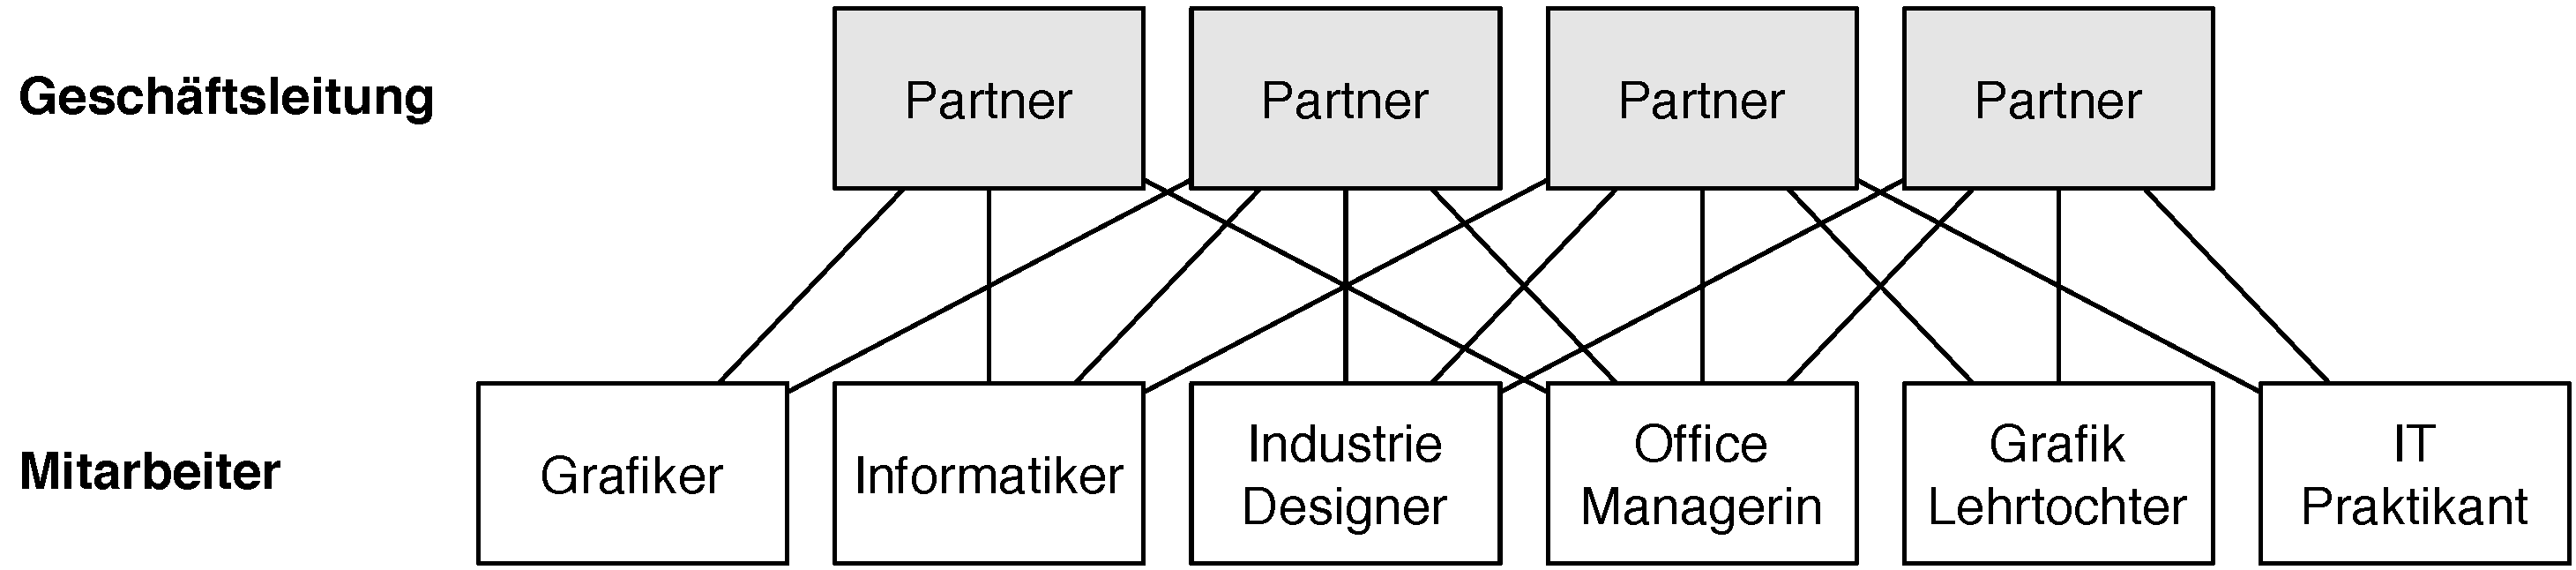
\includegraphics[width=0.95\textwidth,angle=0]{./bilder/ist_organigramm.pdf}
\caption{Aktuelles Organigramm von allink}
\label{pic:ist_organigramm}
\end{center}
\end{figure}

Die Partner kümmern sich um die Projekte, deren Leitung sie übernommen haben
und versuchen anhand den verfügbaren Mitarbeitern und Fachkräften die Projekte 
erfolgreich durchzuführen. Jeder Partner organisiert die benötigten Mitarbeiter
selbst. Dabei kann es vorkommen, dass ein Mitarbeiter parallel an
mehreren Projekten arbeiten muss.

Dies funktioniert so lange gut, bis die Mitarbeiter völlig ausgelastet oder sogar
überbelastet sind. Dies gilt natürlich auch für die Partner. Sobald ein gewisses 
Auftragspensum erreicht ist, kommen die parallel laufenden Projekte ins Stocken 
und schwächen sich gegenseitig. Die Inexistenz eines Projektablaufes bringt
einige Probleme mit sich.

Die Ressourcenüberbelastung ist nur ein Problem, das zum Vorschein kommt. In der
Abbildung \ref{pic:voruntersuchung_projektablauf} verschaffe ich mir einen 
Überblick über die möglichen Gefahren und Schwächen des aktuellen Projektablaufes.

\begin{figure}[htbp]
\begin{center}
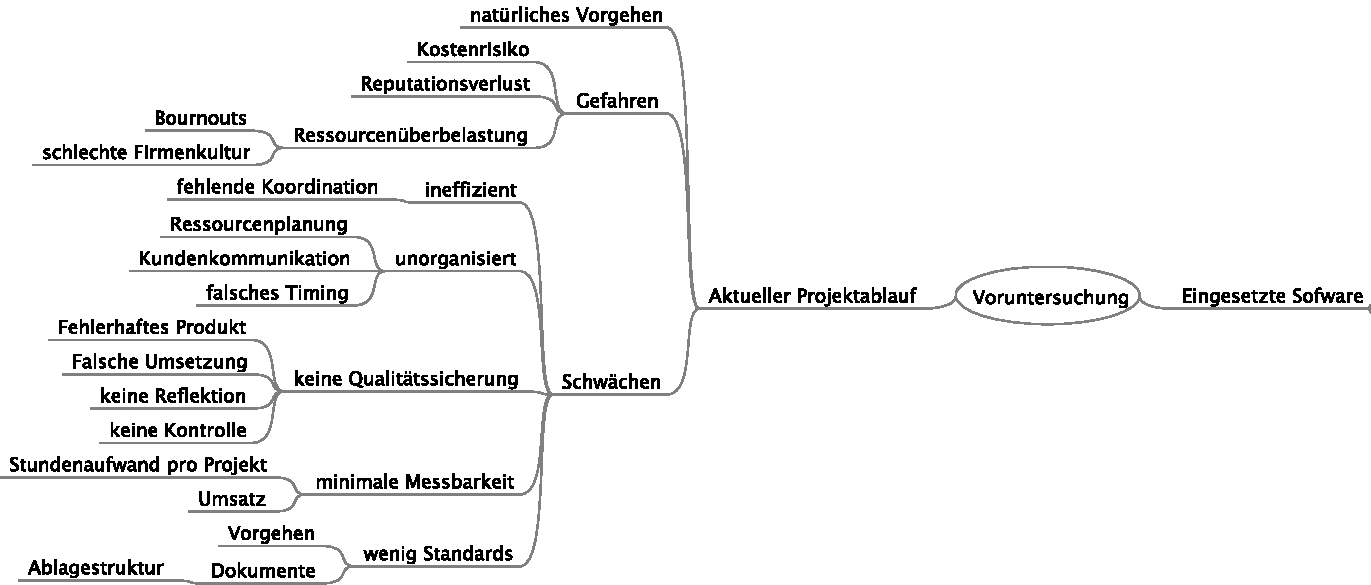
\includegraphics[width=0.95\textwidth,angle=0]{./mindmaps/voruntersuchung_projektablauf.pdf}
\caption{MindMap Voruntersuchung des aktuellen Projektablaufes}
\label{pic:voruntersuchung_projektablauf}
\end{center}
\end{figure}

\subsubsection{Wenig Standards}
Man hält vor, während und nach einem Projekt nur an wenige Standards fest. 
Das ganze Vorgehen ist nicht einheitlich, da in jedem Projekt wieder von
neuem entschieden wird, wie man vorgehen will. Es werden nur wenige einheitlichen
Dokumente verwendet, zum Beispiel für die Erstellung von Offerten und Rechnungen.
Aber auch da entstehen schnell Fehler, z.B. während der Umstellungen des 
Mehrwert Steuersatzes von 7.6\% auf 8\%. Da kein einheitliches Basistemplate
existiert, muss jeder der eine Rechnung schreibt noch einmal sicherstellen, ob
auch der korrekte Steuersatz hinterlegt ist. 

\subsubsection{Unorganisiert}
Durch die Überbelastung können mit der Zeit die versprochenen Timings
nicht mehr eingehalten werden. Da die Ablagestrukturen nicht einheitlich geregelt
sind, kann es vorkommen, dass ein Mitarbeiter einem Kunden ein veraltetes oder
noch nicht freigegebenes Dokument sendet. Dies zieht einen zusätzlichen 
Mehraufwand mit sich, da man sich beim Kunden entschuldigen und rechtfertigen
muss. Zusätzlich strapaziert es auch die Beziehung zum Kunden.

\subsubsection{Ineffizient}
Einfache Abläufe werden so unnötig verkompliziert und aufgehalten. Die ganze
Struktur wird langsam und ineffizient. Was sich wiederum negativ auf die zur
Verfügung stehende Zeit auswirkt.

\subsubsection{Keine Qualitätssicherung}
Oft bleibt gegen Ende eines Projektes dann zu wenig Zeit die nötige 
Qualitätskontrollen durchzuführen, da man sich möglichst schnell um ein anderes,
möglicherweise auch schon überfälliges, Projekt kümmern muss. Der Kunde entdeckt
dann offensichtliche Fehler selbst und zweifelt zwangsläufig an der ganzen Arbeit.

\subsubsection{Minimale Messbarkeit}
Auch bietet die fehlende bzw. chaotische Struktur nur wenige Punkte um Kennzahlen
zu messen. Den Umsatz den man mit dem Projekt erzielt hat ist zwar bekannt,
jedoch kann nur aus dem Gefühl heraus erahnt werden, ob mit dem Projekt einen
Gewinn für die Firma erzielt werden konnte. Die Mitarbeiter sind zwar angehalten
ihre Stunden in ein gemeinsames Stundelog pro Projekt einzutragen, jedoch werden
die Informationen nicht ausgewertet und können nicht mehr einzelnen Mitarbeitern
zugeordnet werden.

\subsubsection{Kostenrisiko}
Durch die fehlende Kontrolle während eines Projektes, verliert man die
Übersicht über die Aufwände und schlussendlich die Kosten. Dadurch entsteht
ein Kostenrisiko, welches Konsequenzen für die Liquidität von allink haben könnte.

\subsubsection{Ressourcenüberbelastung}
Die Belastung für den Mitarbeiter wie auch für die Partner ist so über
längere Zeit nicht tragbar. Durch eine Überarbeitung kann es zu Ausfällen kommen, die
die Situation zusätzlich verschlimmern könnten. Das ganze Endet in einer 
schlechten Firmenkultur und das Unternehmung beginnt von innen zu zerfallen.

\subsubsection{Reputationsverlust}
Da man Timings nicht mehr einhalten kann und man sich gegenüber dem Kunden
oft rechtfertigen muss entsteht ein schlechtes Bild der Unternehmung und sie
verliert an Vertrauen. Da die Konkurrenz im Tätigkeitsfeld der allink relativ
gross ist, ist ein möglicher Absprung und Angenturwechsel seitens des Kunden nicht 
auszuschliessen.

\subsection{Zurzeit eingesetzte Software}
Bei der Untersuchung der zur Zeit eingesetzten Sofware beschränke ich mich auf jene,
die einen direkten Einfluss auf den aktuellen Projektablauf bei allink haben.
Ich liste keine Software auf, die zur Erbringung der eigentlichen Dienstleistungen
von allink eingesetzt werden.

\begin{figure}[htbp]
\begin{center}
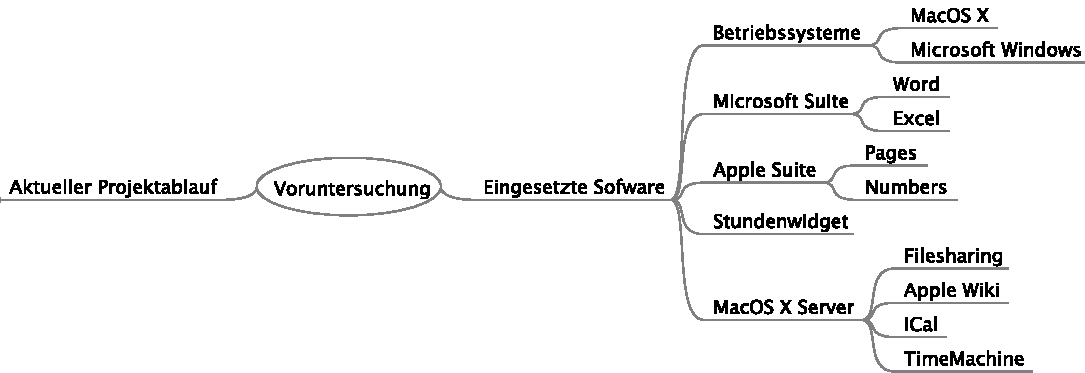
\includegraphics[width=0.95\textwidth,angle=0]{./mindmaps/voruntersuchung_software.pdf}
\caption{MindMap Voruntersuchung der eingesetzten Software}
\label{pic:voruntersuchung_software}
\end{center}
\end{figure}

\subsubsection{Betriebssysteme}
Als Hauptbetriebssystem verwendet allink Mac OS X\footnote{Betriebssystem von Apple \url{http://www.apple.com/macosx/}}.
Es läuft auf allen Arbeitsstationen der Mitarbeiter und Partner. Zusätzlich haben einige der
Entwickler noch Microsoft Windows\footnote{Betriebssystem von Microsof \url{http://www.microsoft.com/windows/}}
über eine Virtualisierungslösung installiert. Dies wird zu Testzwecken benötigt.

\subsubsection{Microsoft Suite}
Da viele Kunden mit Microsoft Produkten arbeiten benötigt auch allink die
Office Suite\footnote{Microsoft Office für Mac \url{http://www.microsoft.com/germany/mac}}, 
um Dateien mit Kunden ohne Interoperabilitätsprobleme
austauschen zu können. Nicht jede Arbeitsstation verfügt zur Zeit über eine
Installation.

\subsubsection{Apple Suite}
Für interne Zwecke setzt allink zur Zeit auf die Apple eigene Office Suite
iWork\footnote{Office Suite von Apple \url{http://www.apple.com/de/iwork/}}.
Pages wird zur Erstellung von Offerten und Rechnungen verwendet. Mit Numbers
werden Tabellenkalkulationen wie die Liquiditätsplanung oder Lohnblätter erstellt.
Da dies aber lange nicht so von der Geschäftsleitung kommuniziert wurde, existieren
auch einige Excel Files, das Pendant der Microsoft Office Suite.

\subsubsection{Stundenwidget}
Das Stundenwidget ist eine selbst geschriebene Software von allink und läuft
im Dashboard\footnote{Widget Lösung von Apple \url{http://www.apple.com/downloads/dashboard/}} des Betriebssystems.
Es ermöglicht Stunden auf ein Projekt zu buchen, wie man auf dem Screenshot \ref{pic:ist_widget}
sehen kann.

\begin{figure}[htbp]
\begin{center}
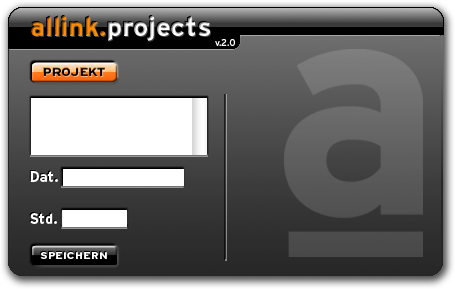
\includegraphics[width=0.55\textwidth,angle=0]{./bilder/ist_widget.png}
\caption{Aktuelles Stundenwidget von allink}
\label{pic:ist_widget}
\end{center}
\end{figure}

Die Daten werden auf dem
eigenen Server gespeichert und pro Projekt abgelegt. Dieses Widget ist auf allen
Arbeitsstationen installiert und wird von den Mitarbeitern gelegentlich verwendet
um ihre Stunden auf ein Projekt zu rapportieren.

\subsubsection{MacOS X Server}
Auf dem Server liegt das zentrale Dateiablagesystem. Die Zugriffsrechte können
auf dem Server für jede Freigabe definiert werden. So haben zum Beispiel
die Mitarbeiter keinen Zugriff auf den Administrationsordner der Geschäftsleitung.
Über diesen Server laufen auch die einzelnen Firmenkalender der Partner. Sie
können so gemeinsam Termine buchen und haben stets Einblick in die anderen
Kalender.

\section{Ist-Aufnahme}
\subsection{Projektablauf}
Zur Zeit existiert bei allink auch kein offizieller Projektablauf. Ich bezeichne
den heutigen Zustand als ``natürliches Vorgehen''. Ein mögliches Projekt
kommt an einen Partner heran, entweder über eine Anfrage oder eine Akquisition,
er spricht sich wenn nötig mit den anderen Partner ab und nimmt dann die
Mitarbeiter mit in das Projekt, die er als nötig erachtet.

\subsubsection{Projektannahme und Offertenerstellung}
In der nachfolgenden Darstellung \ref{pic:01_ist_prozesse_offerte} ist der
aktuelle Prozess der Offertenerstellung ersichtlich. Die darin verwickelten
Akteuere sind der Kunde und der bzw. die Partner.

\begin{figure}[htbp]
\begin{center}
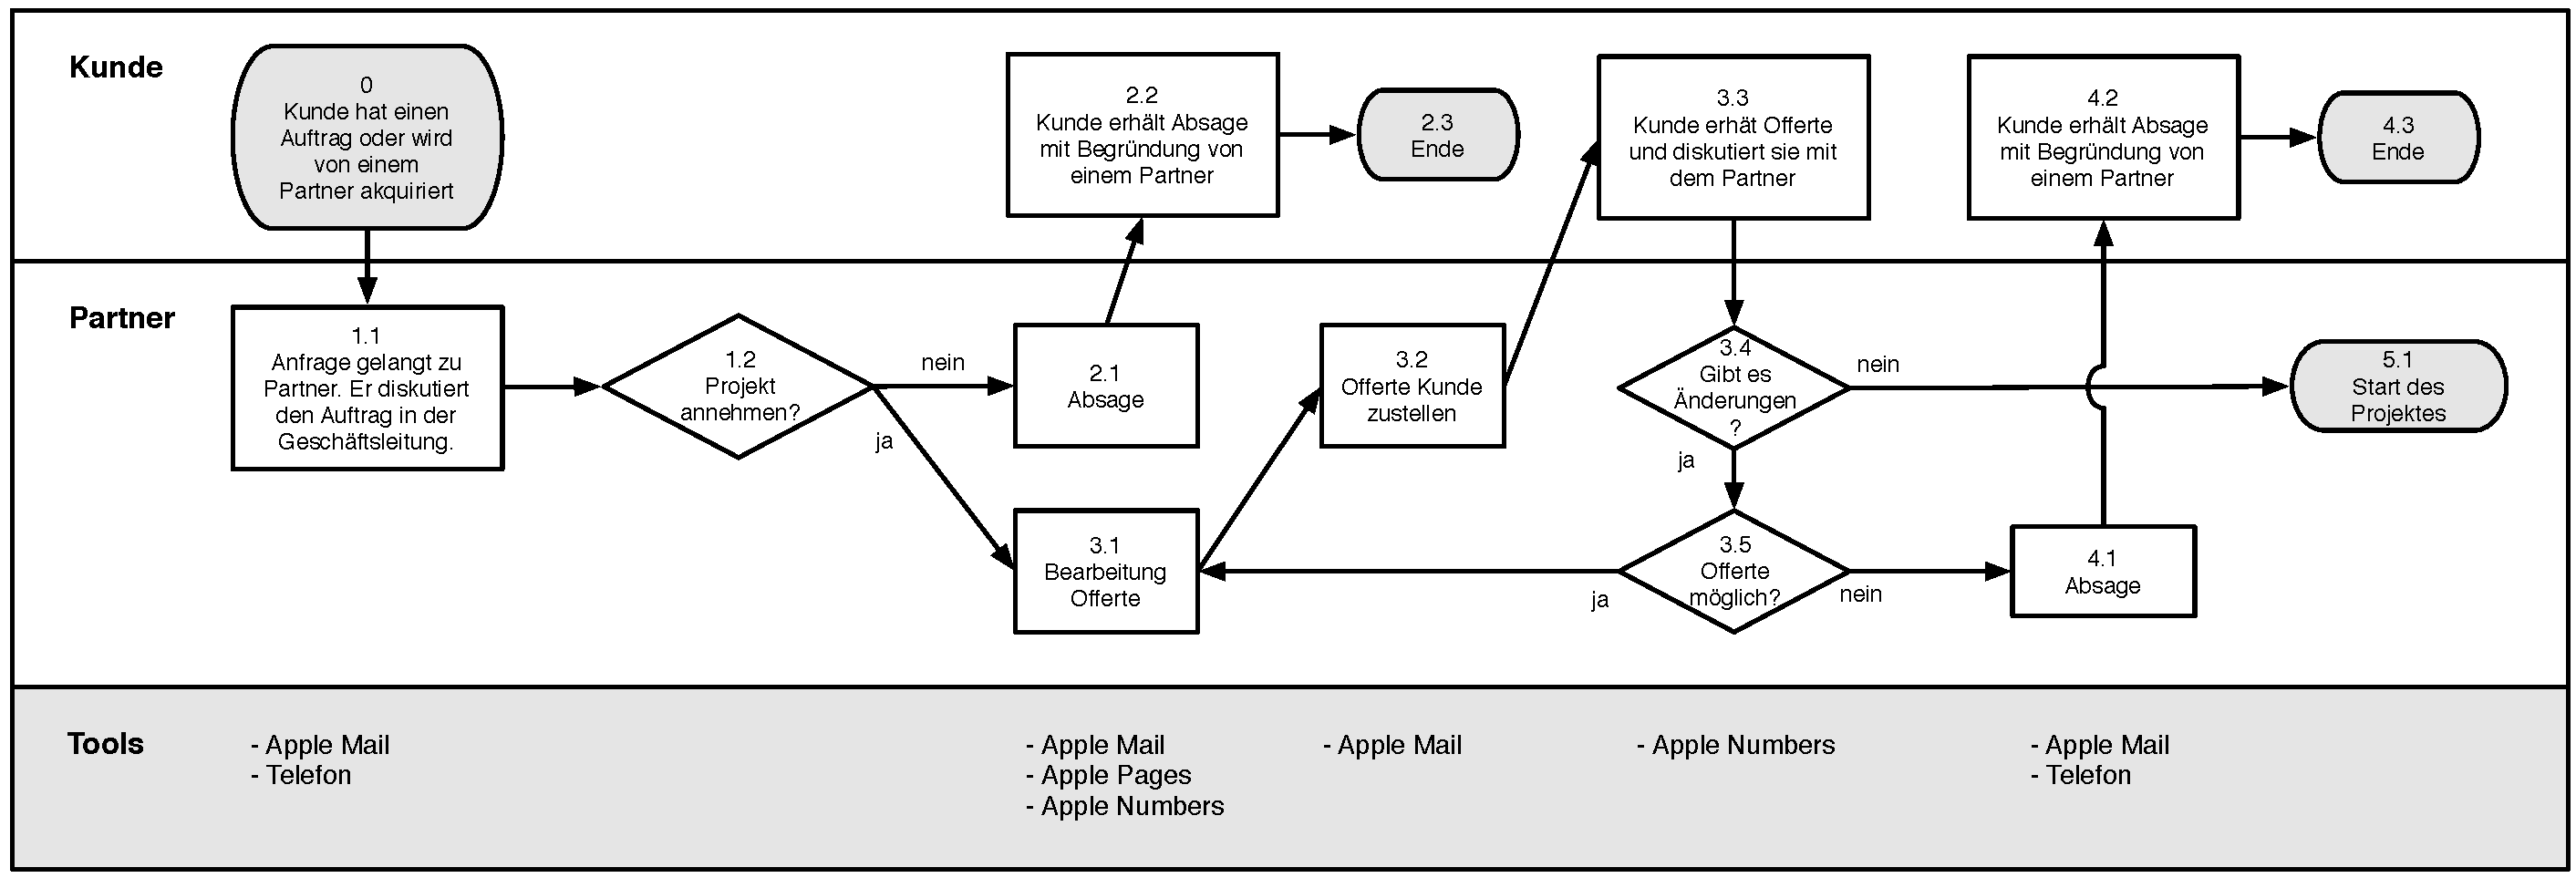
\includegraphics[width=0.99\textwidth,angle=0]{./bilder/01_ist_prozesse_offerte.pdf}
\caption{Offertenerstellungs Prozess von allink März 2011}
\label{pic:01_ist_prozesse_offerte}
\end{center}
\end{figure}

Detaillierte Beschreibung des Prozesses.

Die Anfrage endet entweder in einer Absage oder einem Start eines neuen 
Projektes. Wenn das Projekt nicht zustande kommt, werden die Aufwände der
Akquisition und der Offertenerstellung zurzeit vernachlässigt und somit von
den übrigen Projekten getragen.

\clearpage

\subsubsection{Projektdurchführung}
Einleitungstext...

\begin{figure}[htbp]
\begin{center}
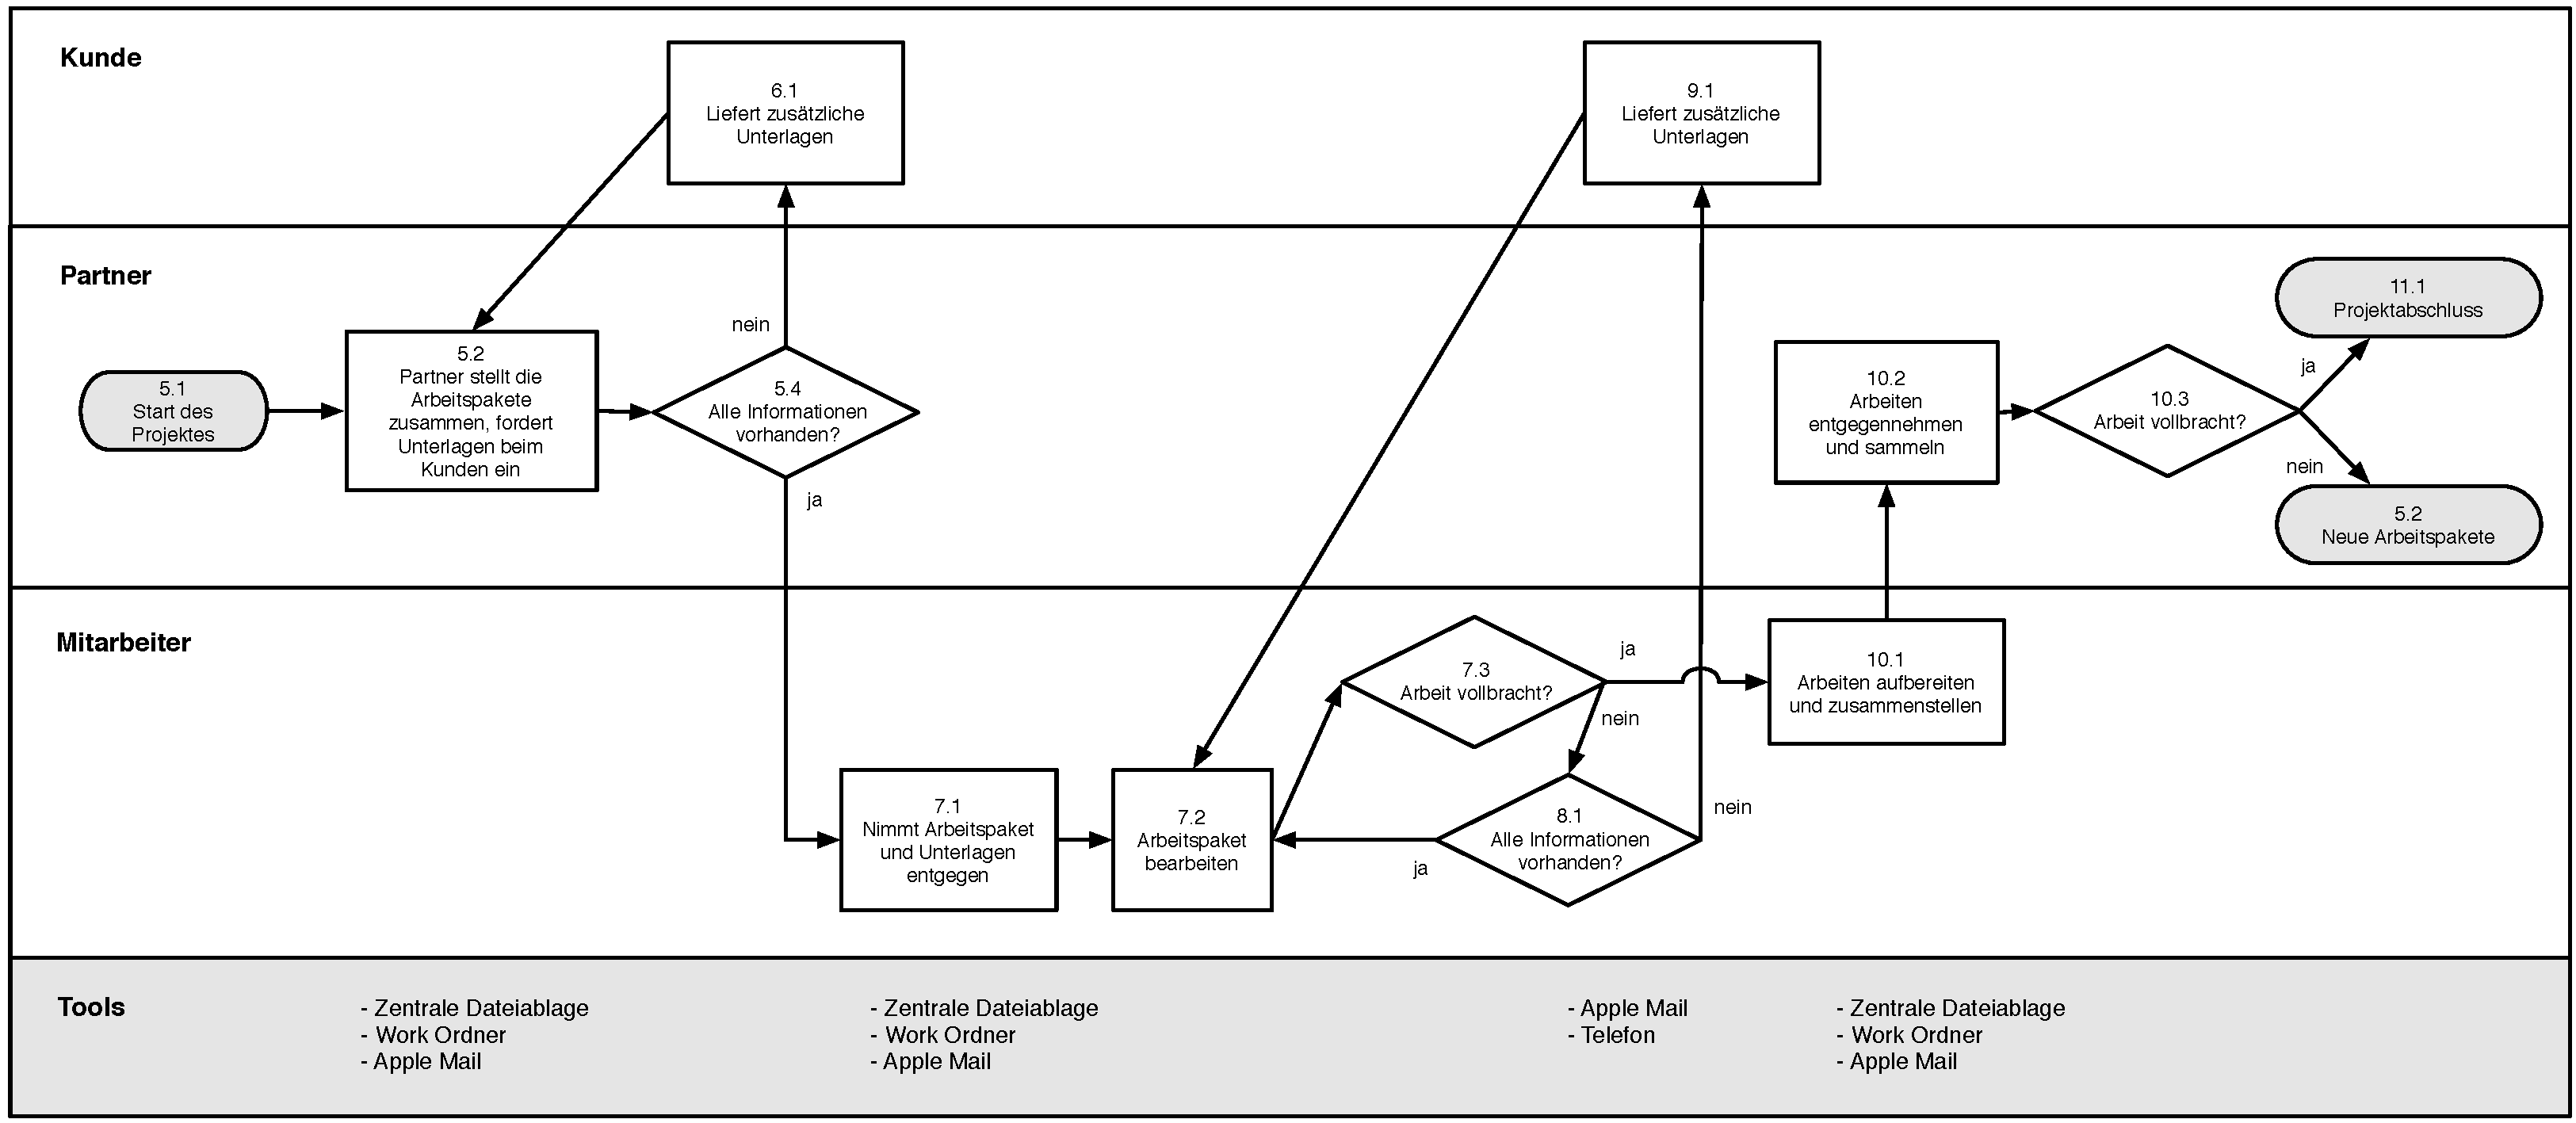
\includegraphics[width=0.99\textwidth,angle=0]{./bilder/02_ist_prozesse_arbeit.pdf}
\caption{Projektumsetzungs Prozess von allink März 2011}
\label{pic:02_ist_prozesse_arbeit}
\end{center}
\end{figure}

Detaillierte Beschreibung des Prozesses...

\clearpage

\subsubsection{Projektabschluss}
Einleitungstext...

\begin{figure}[htbp]
\begin{center}
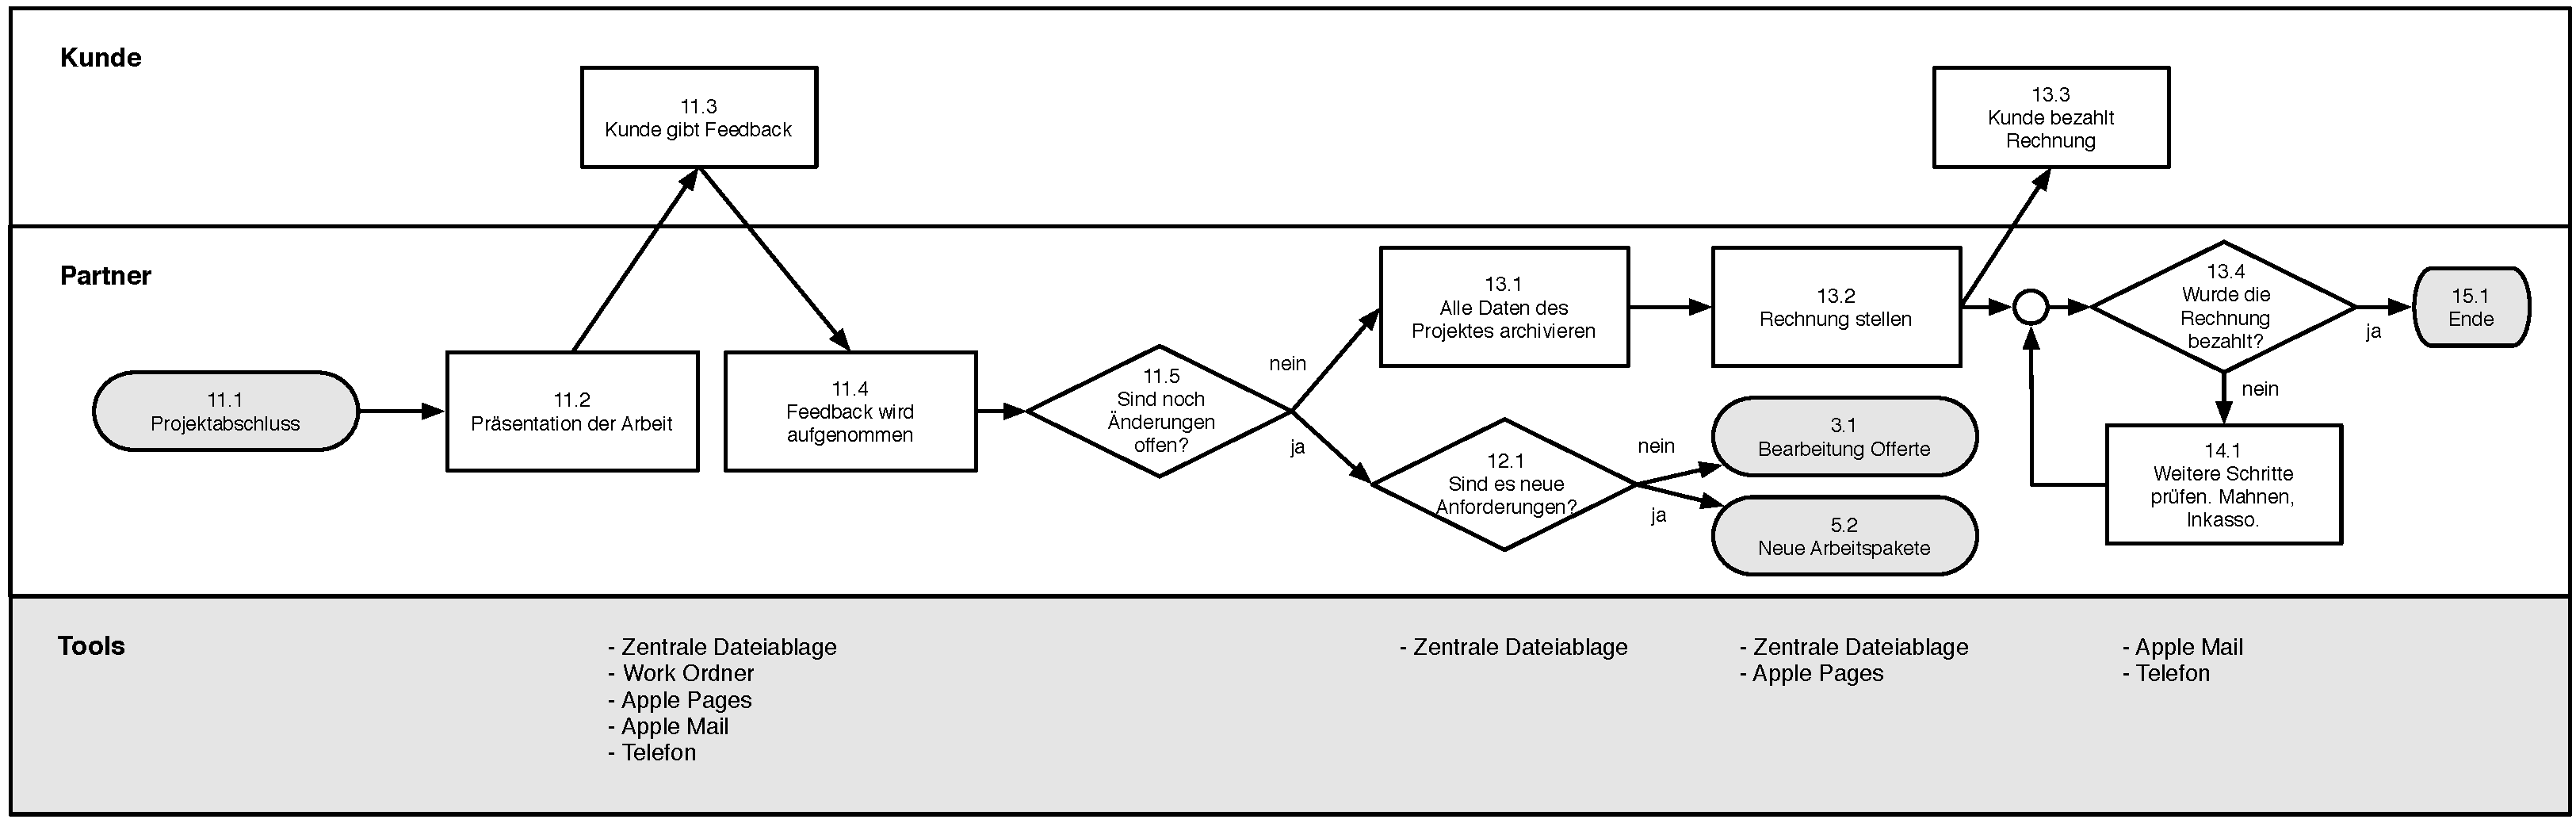
\includegraphics[width=0.99\textwidth,angle=0]{./bilder/03_ist_prozesse_abschluss.pdf}
\caption{Projektabschluss Prozess von allink März 2011}
\label{pic:03_ist_prozesse_abschluss}
\end{center}
\end{figure}

Detaillierte Beschreibung des Prozesses...

\section{Ist-Kritik}
Problem-Ursachen Matrix

\section{Konklusion}
  \cleardoublepage
  
  \chapter{Anforderungen}
  \section{Stakeholder}
  \subsection{Kunde}
  \subsection{Partner}
  \subsection{Mitarbeiter}
  \subsection{Drittanbieter}
  \section{Nicht funktionale Anforderungen}
  \section{Funktionale Anforderungen}
  \section{Kennzahlen}
  
  \chapter{Konzept}
  \section{Varianten}
  \subsubsection{Variante 1}
  \subsubsection{Variante 2}
  \subsubsection{Variante 3}
  \section{Nutzwertanalyse}
  
  \chapter{Proof of Concept}
  
  \chapter{Reflektion}
  \section{Fazit}
  \section{Ausblick}
  \section{Danksagung}
  
  \appendix
  
  \chapter{Personalienblatt}
  \begin{tabbing}
	\hspace*{4cm}   \= \kill
	Name, Vorname:  \> {\bf Spross, Silvan} \\
	Adresse:        \> {\bf Meinrad Lienert-Strasse 27} \\
	PLZ, Wohnort:   \> {\bf 8003 Zürich} \\
	\\
	Geburtsdatum:   \> {\bf 07.11.1985} \\
	Heimatort:      \> {\bf Zürich ZH} \\
\end{tabbing}

  
  \chapter{Bestätigung}
  Hiermit bestätige ich, Silvan Spross, dass die vorliegende Diplomarbeit 
``Definition und Optimierung der Projektprozesse bei allink.creative'' im
Rahmen der geltenden Reglemente und in allen Teilen selbständig erarbeitet und 
durchgeführt wurde.\\
\\
Zürich, den 31. Mai 2011\\
\\\\
Silvan Spross
  
  \listoffigures
  \listoftables
  %\lstlistoflistings
  
  \bibliographystyle{alpha}
  \bibliography{literaturverzeichnis}
  
  \chapter{Rahmenbedingungen}
  Für das Informatik Diplomstudium an der Fachhochschule Zürich für Technik
HSZ-T wird von den Studenten verlangt eine Diplomarbeit eigenständig zu
verfassen.

\section{Sprache}
Die Semesterarbeit wurde in deutscher Sprache verfasst. Englische Ausdrücke 
wurden immer dort verwendet, wo diese im Sprachgebrauch in den verwendeten 
Programmen genau so gebraucht werden.

Aus Gründen der besseren Lesbarkeit der Diplomarbeit wurde teilweise auf 
die Nennung beider Geschlechter verzichtet. In diesen Fällen ist die 
weibliche Form ausdrücklich inbegriffen.
  
\section{Richtlinien}
Folgende Dokumente mit Richtlinien der Hochschule für Technik Zürich 
wurden für die Diplomarbeit berücksichtigt:

\begin{itemize}
    \item Reglement \cite{hsz_reglement}
    \item Ablauf \cite{hsz_ablauf}
    \item Bewertungskriterien \cite{hsz_bewertungskriterien}
\end{itemize}

  \cleardoublepage
  
  \chapter{Aufgabenstellung}\label{chap:aufgabenstellung}
  \section{Ausgangslage}
Die Agentur allink.creative ist im letzten Jahr stark gewachsen. Von zehn
Mitarbeitern im Februar 2010 auf siebzehn Mitarbeiter im Februar 2011. Dies hat 
zur Auswirkung, dass gewisse Funktionen und Prozesse neu definiert und bestehende
überarbeitet werden müssen, um weiterhin effizient, oder wenn möglich noch 
effizienter, arbeiten zu können. Die Agentur arbeitet überwiegend mit Apple
Computern und setzt gewisse Software ein, die die Geschäftsleitung beibehalten 
möchte. Die konkreten Vorstellungen und Vorgaben müssen in dieser Arbeit erfasst 
werden.

\section{Ziel der Arbeit}
Bereiche wie die Stundenrapportierung, die Projektplanung und das Projektcontrolling 
können mit Hilfe von IT-Lösungen massgebend optimiert und vereinfacht werden. 
In dieser Arbeit sollen die Herausforderungen, die der Auftraggeber in der 
Planung und im Controlling eines Projektes zu bewältigen hat, erfasst und 
Lösungsvorschläge evaluiert werden. Der Fokus liegt dabei auf der besseren 
Messbarkeit des finanziellen Erfolges eines Projektes und des gesamten 
Unternehmens.

Die Arbeit grenzt sich ganz klar von der Finanzbuchhaltung ab, da
diese keinen direkten Einfluss auf die Projekte hat und bei allink.creative 
bei einen Treuhänder ausgelagert wurde.

\section{Aufgabenstellung}
Folgende Aufgaben soll der Studierende während dieser Arbeit bewältigen:

\begin{itemize}
    \item Ist-Situation im Bereich Projektablauf der allink.creative erfassen
    \item Kennzahlen definieren, die in Zukunft auf Projektebene gemessen 
        werden sollen
    \item Eine Recherche der Prozesse in ähnlich funktionierenden KMUs durchführen
    \item Neue Prozesse definieren und bestehende, sofern sinnvoll, überarbeiten
    \item Evaluation von IT-Lösungen, die diese Prozesse möglichst passend 
        für den Auftraggeber abbilden und die definierten Kennzahlen generieren können
\end{itemize}

\section{Erwartete Resultate}
Der Studierende soll dem Auftraggeber ein Dokument erstellen, das folgende 
Punkte beinhaltet: 

\begin{itemize}
    \item Beschreibung der Ist-Situation im Bereich Projektablauf
    \item Übersicht der bestehenden Software beim Auftraggeber
    \item Kennzahlen, die auf Projektebene gemessen werden sollen
    \item Darstellung der neuen und überarbeiteten Prozesse
    \item Übersicht der bestehenden Software in der neuen Prozesslandschaft
    \item Softwareempfehlungen für die komplette Prozessabbildung
    \item ``Make or Buy''-Entscheid mit dem Auftraggeber
\end{itemize}

Während der Arbeit sollen als ``Proof of Concept'' die selben zur Zeit verwendeten
Prozesse und Tools verwendet werden. Sobald die neuen Prozesse und Tools
definiert sind und der Auftraggeber einen Entscheid gefällt hat, sollen die
Informationen ebenfalls in die neue Prozess- und Toollandschaft übertragen werden.

\section{Abgrenzung}
Folgende Punkte werden abgegrenzt, da sie den Rahmen der Arbeit Überschreiten 
würden:

\begin{itemize}
    \item Die Analysen beschränken sich auf Recherchen im Internet und Büchern
    \item Umfragen, Erhebungen sowie Feldstudien werden nicht durchgeführt
\end{itemize}


  \cleardoublepage
  
  \section{Detailanalyse der Aufgabenstellung}
In der Detailanalyse der Aufgabenstellungen formuliere ich die zu bewältigenden
Aufgaben und deren erwartete Resultate aus.

\subsection{Zu bewältigende Aufgaben}
\subsubsection{Ist-Situation im Bereich Projektablauf der allink.creative erfassen}
Es soll eine Beschreibung des aktuellen Projektablaufes der allink erarbeitet
und möglichst vollständig alle heutigen Prozessschritte dargestellt und die Vor- 
und Nachteile des Projektablaufes aufgezeigt werden. Hinzu kommt die darin verwendete Software und
deren Einsatzzweck.
\\\\
\underline{Erwartete Resultate}

\begin{description}
    \item[R1] Beschreibung der Ist-Situation im Bereich Projektablauf
    \item[R2] Übersicht der bestehenden Software beim Auftraggeber
\end{description}

\subsubsection{Kennzahlen definieren, die in Zukunft auf Projektebene gemessen werden sollen}
Zusammen mit dem Auftraggeber sollen Voraussetzungen, unteranderem Kennzahlen,
definiert werden, die bei der Erarbeitung des neuen Projektablaufes berücksichtig
werden müssen. 
\\\\
\underline{Erwartete Resultate}

\begin{description}
    \item[R3] Kennzahlen, die auf Projektebene gemessen werden sollen
\end{description}
  
\subsubsection{Eine Recherche der Prozesse in ähnlich funktionierenden KMUs durchführen}
Der Studierende soll in Gesprächen mit anderen KMUs recherchieren, was Agenturen
mit ähnlichen Voraussetzungen und Herausforderungen wie allink für Projektabläufe
und Hilfsmittel verwenden.
\\\\
\underline{Erwartete Resultate}

Die Informationen aus den Recherchen sollen in den Lösungsvorschlag eingearbeitet
und berücksichtigt werden.

\subsubsection{Neue Prozesse definieren und bestehende, sofern sinnvoll, überarbeiten}
Anhand den bis dahin gewonnen Erkenntnissen soll der bestehende Projektablauf
überarbeitet und neu definiert werden. Dazu arbeitet der Studierende eng mit
dem Auftraggeber zusammen, damit sichergestellt ist, dass eine in der Realität
umsetzbare Lösung definiert wird.
\\\\
\underline{Erwartete Resultate}

\begin{description}
    \item[R4] Darstellung der neuen und überarbeiteten Prozesse
    \item[R5] Übersicht der bestehenden Software in der neuen Prozesslandschaft
    \item[R6] Softwareempfehlungen für die komplette Prozessabbildung
\end{description}

\subsubsection{Evaluation von IT-Lösungen, die diese Prozesse möglichst passend 
    für den Auftraggeber abbilden und die definierten Kennzahlen generieren können}
Sofern die bestehende Software des Auftraggebers nicht ausreicht um den neuen
Projektablauf im Unternehmen umzusetzen, soll der Studierende alternative 
Lösungen evaluieren. Darin können auch selbst umzusetzende Tools empfohlen 
werden, sofern der Aufwand für dessen Entwicklung gerechtfertigt ist.
\\\\
\underline{Erwartete Resultate}

\begin{description}
    \item[R7] ``Make or Buy''-Entscheid mit dem Auftraggeber
\end{description}

\section{Aufwandschätzung}
Aufgrund den Anforderungen an eine Diplomarbeit und aus der Aufgabenstellung
ergeben sich für mich Arbeitspakete, die ich in eine Planungs- und Umsetzungsphase
der Diplomarbeit unterteile. Auch versuche ich den Aufwand der einzelnen
Arbeitspaketen in Stunden zu schätzen und diese dann in eine realistische 
Projektplanung einfliessen zu lassen.

\subsection{Planungsphase}
Die Arbeitspakete, die vor der Freigabe der Diplomarbeit erbracht werden müssen,
sind in Stunden geschätzt und in der Tabellen \ref{tab:auwand_planungsphase} 
aufgelistet.

\begin{table}[h]
\begin{center}
    \begin{tabular}{llc}
        \toprule & \textbf{Arbeitspaket} & \textbf{Aufwand in Stunden} \\
        \midrule \textbf{P1} & Thema evaluieren & 16 \\
        \midrule \textbf{P2} & Aufgabenstellung ausarbeiten & 20 \\
        \midrule \textbf{P3} & Betreuer finden & 16 \\
        \midrule \textbf{P4} & Kick-Off vorbereiten & 12 \\
        \bottomrule & \textbf{Total Stunden} & \textbf{64} \\
        \bottomrule
    \end{tabular}
    \caption{Aufwandschätzung der Arbeitspakete der Planungsphase}
    \label{tab:auwand_planungsphase}
\end{center}
\end{table}

\subsection{Umsetzungsphase}
Die Arbeitspakete, die während der Diplomarbeit erbracht werden müssen, sind
in Stunden geschätzt und in der Tabelle \ref{tab:aufwand_umsetzungsphase}
aufgelistet.

\begin{table}[h]
\begin{center}
    \begin{tabular}{llc}
        \toprule & \textbf{Arbeitspaket} & \textbf{Aufwand in Stunden} \\
        \midrule \textbf{P5} & Ist-Situation erfassen & 40 \\
        \midrule \textbf{P6} & Kennzahlen definieren & 28 \\
        \midrule \textbf{P7} & Review vorbereiten & 12 \\
        \midrule \textbf{P8} & Prozesse definieren und überarbeiten & 44 \\
        \midrule \textbf{P9} & Evaluation von IT Lösungen & 28 \\
        \midrule \textbf{P10} & Abschluss Arbeit & 16 \\
        \midrule \textbf{P11} & Druckauftrag & 12 \\
        \midrule \textbf{P12} & Vorbereitung Präsentation & 16 \\
        \bottomrule & \textbf{Total Stunden} & \textbf{196} \\
        \bottomrule
    \end{tabular}
    \caption{Aufwandschätzung der Arbeitspakete der Umsetzungsphase}
    \label{tab:aufwand_umsetzungsphase}
\end{center}
\end{table}

\section{Projektplan}
Den provisorischen Projektplan erstelle ich aufgrund den geschätzten Aufwände
und den vorgegebenen Terminen der HSZ-T. Die gewählten Termine der Meilensteine
``Abgabe Diplomarbeit'' und ``Präsentation Diplomarbeit'' sind meine Wunschtermine
und noch nicht offiziell bestätigt.

Das Total der zu bewältigenden und geschätzten Stunden beläuft sich 
auf 260 Stunden. Diese versuche ich möglichst realistisch über den mir noch
zur Verfügung stehenden Zeitraum zu verteilen. Dies habe ich mit Hilfe der 
Projektplanungs-Software Merlin\footnote{\url{http://www.projectwizards.net/de/merlin/}} 
erstellt und eine Übersicht ist in der unten stehenden Grafik \ref{pic:projektplan} 
dargestellt.

\begin{figure}[htbp]
\begin{center}
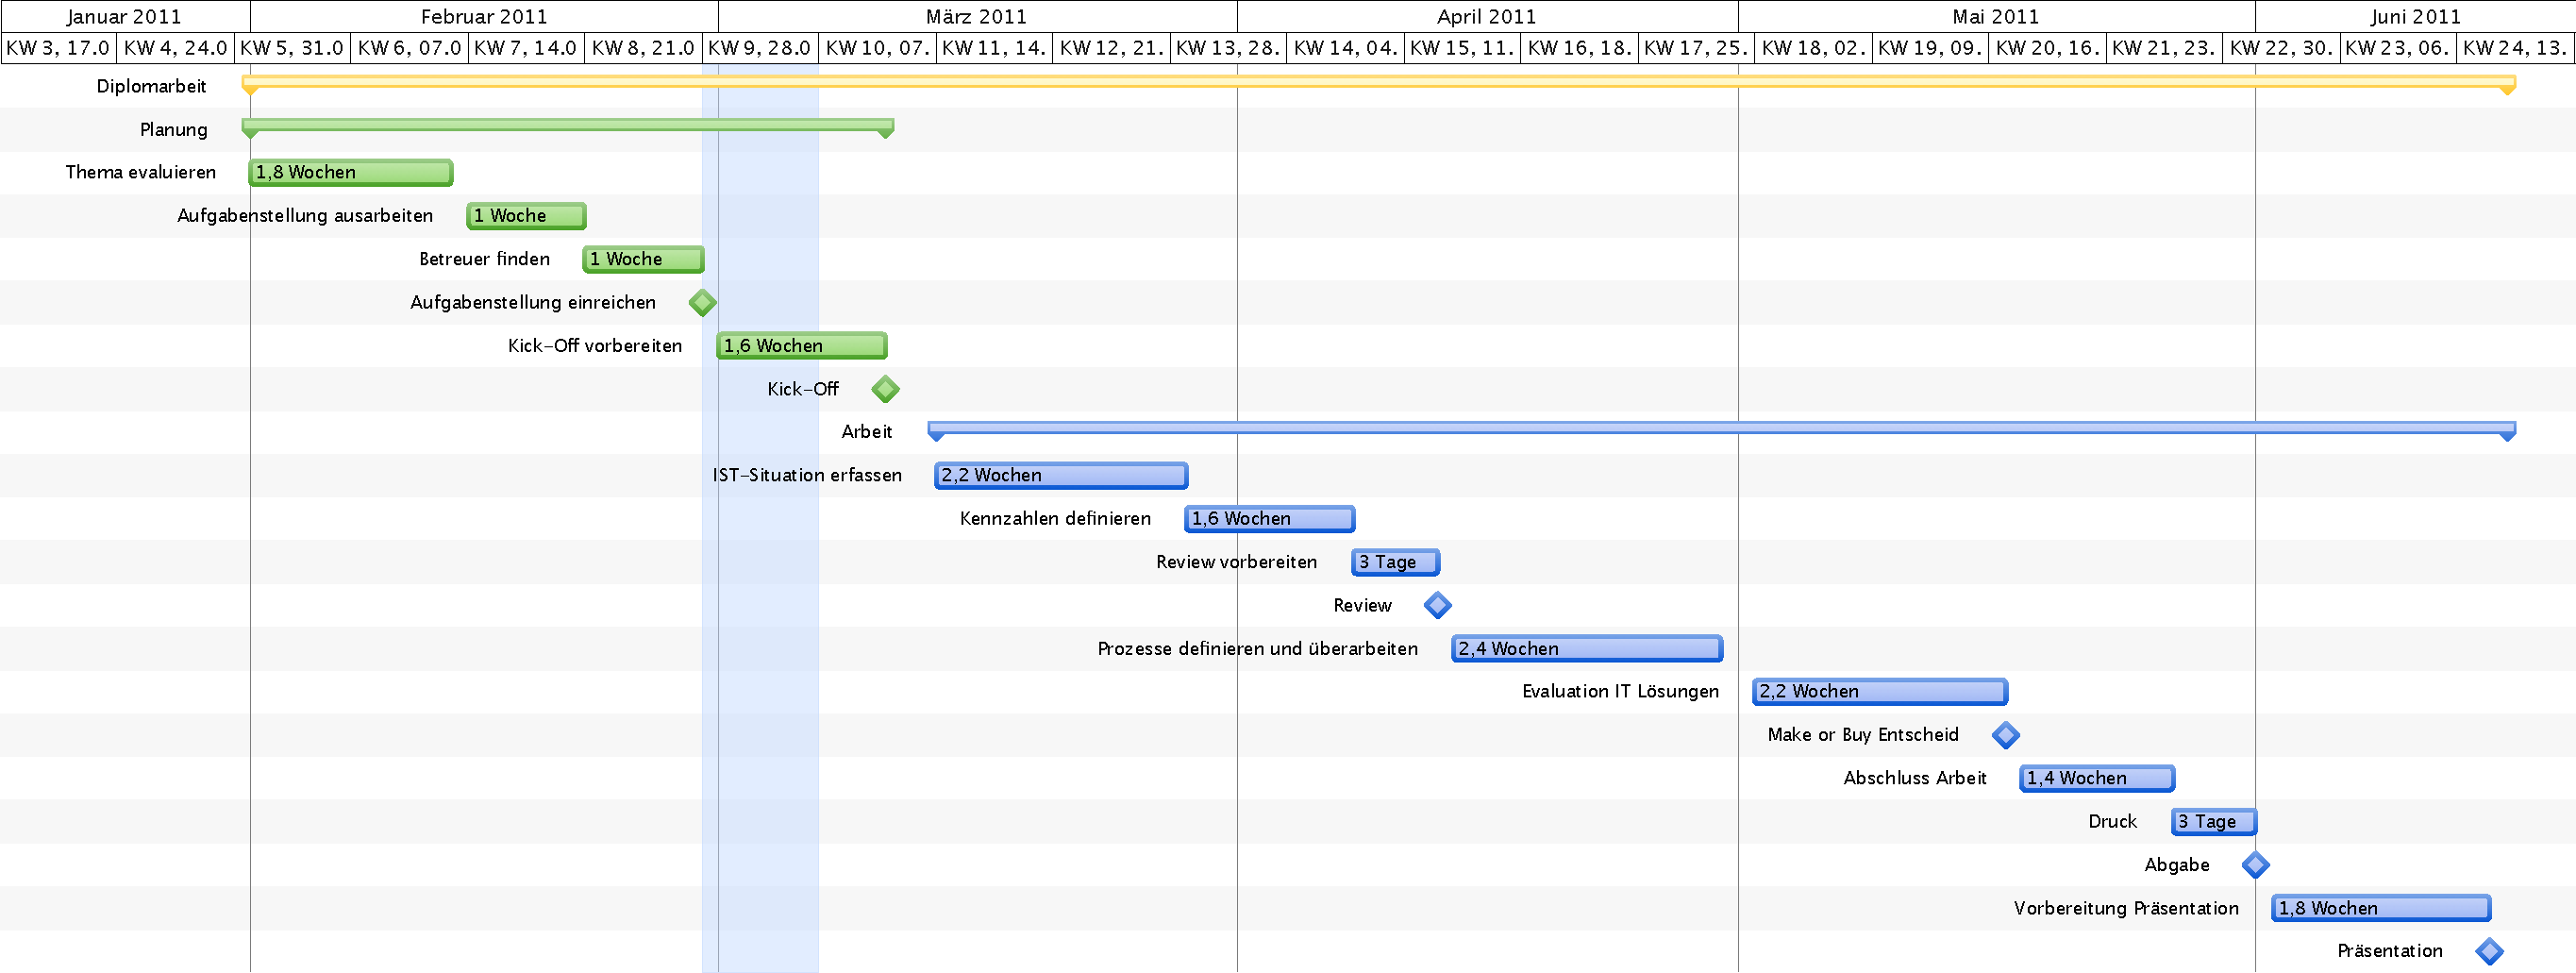
\includegraphics[width=1\textwidth,angle=0]{./bilder/projektplanung.pdf}
\caption{Projektplan der Diplomarbeit aus Merlin}
\label{pic:projektplan}
\end{center}
\end{figure}

Ich bin mir bewusst, dass es eine eher optimistische Projektplanung ist. Jedoch
steht mir, aus administrativen Gründen der HSZ-T, nur noch dieser Zeitraum für
die Durchführung der Diplomarbeit übrig um mein Studium erfolgreich abschliessen
zu können. Trotz der optimistischen Planung bin ich zuversichtlich, diese
im gegebenen Zeitrahmen umsetzen und abschliessen zu können.

Zum Zeitpunkt des Designreviews werde ich anhand des bisherigen Projektverlaufes
die Situation neu beurteilen und, wenn nötig, die Planung überdenken und 
gegebenenfalls anpassen.

\section{Termine}
In der Tablle \ref{tab:termine_diplomarbeit} sind alle Termine, die sich aus 
dem Projektplan, den bekannten Terminen und Wunschterminen ergeben, in chronologischer
Reihenfolge ihrer Durchführung aufgelistet.

Zusätzlich habe ich sie mit den abhängenden Arbeitspaketen
und Resultaten ergänzt, die zum Zeitpunkt des Termins vorhanden und erfüllt
sein sollten.

\begin{table}[h]
\begin{center}
    \begin{tabular}{llll}
        \toprule & & \multicolumn{2}{c}{\textbf{Abhängende}} \\
        \textbf{Datum} & \textbf{Termin} & \textbf{Arbeitspakete} & \textbf{Resultate} \\
        \midrule 28.02.2011 & Aufgabenstellung einreichen & P1, P2, P3 & - \\
        \midrule 11.03.2011 & Kick-Off Meeting & P4 & -\\
        \midrule 13.04.2011 & Review Termin & P5, P6, P7 & R1, R2, R3 \\
        \midrule 17.05.2011 & ``Make or Buy''-Entscheid & P8, P9 & R4, R5, R6 \\
        \midrule 01.06.2011 & Abgabe Diplomarbeit & P10, P11 & R7 \\
        \midrule 15.06.2011 & Präsentation Diplomarbeit & P12 & - \\
        \bottomrule
    \end{tabular}
    \caption{Auflistung der Termine der Diplomarbeit}
    \label{tab:termine_diplomarbeit}
\end{center}
\end{table}

\section{Erreichte Ziele}
In der nachfolgenden Tabelle \ref{tab:erreichte_ziele} sind alle Ziele gemäss 
den erwarteten Resultaten der Aufgabenstellung aufgelistet. Alle 
erwarteten Ziele wurden erreicht.


\begin{center}
    \begin{longtable}{p{8cm}lcl}
        \toprule \textbf{Ziel} & \textbf{Resultat} & \textbf{Stand} \\
        \midrule Die Ist-Situation im Bereich Projektablauf der allink.creative
            ist beschrieben und abgebildet. & R1 & noch nicht erfüllt \\
        \midrule Eine Übersicht über die bestehende Software bei allink.creative
            wurde erstellt. & R2 & noch nicht erfüllt \\
        \midrule Die Kennzahlen, die auf Projektebenen gemessen werden sollen,
            wurden definiert. & R3 & noch nicht erfüllt \\
        \midrule Die neuen und überarbeiteten Prozesse sind beschrieben und
            abgebildet. & R4 & noch nicht erfüllt \\
        \midrule Eine Übersicht über die bestehende Software bei allink.creative
            in der neuen Prozesslandschaft wurde erstellt. & R5 & noch nicht erfüllt \\
        \midrule Eine Softwareempfehlung für die komplette Prozessabbildung
            wurde erstellt und begründet. & R6 & noch nicht erfüllt \\
        \midrule Ein ``Make or Buy''-Entscheid wurde mit dem Auftraggeber 
            getroffen und festgehalten. & R7 & noch nicht erfüllt \\
        \bottomrule
        \caption{Auflistung der erwarteten Resultate mit Stand der Erfüllung}
        \label{tab:erreichte_ziele}
    \end{longtable}
\end{center}

  \cleardoublepage
  
  \chapter{Protokolle}
  \section{Kick-Off Protokoll}
  \section{Design Review Protokoll}
  \section{Arbeitsprotokoll}

\end{document}